\subsection{La tecnologia Bootstrap}

    \paragraph{}
    Bootstrap és el marc de treball o `framework', més popular pels llenguatges HTML, CSS i Javascript de cara a desenvolupar aplicacions web de disseny adaptatiu i aplicacions web orientades a dispositius mòbils.

    Bootstrap proporciona un conjunt d'estils CSS i codis Javascript que faciliten el desenvolupament de certes funcionalitats per les aplicacions web.

    La funcionalitat principal que va portant-se a decidir utilitzar aquesta tecnologia és la funcionalitat del grid o quadrícula. A l'hora de programar una pàgina web que vol ser pintada de forma apropiada tant en dispositius mòbils com escriptoris, un dels punts més complicats és el d'assegurar que tots els components definits es comportaran com s'espera d'ells en cada dispositiu i que ocuparan posicions diferents segons la grandària del dispositiu en què es mostren.

    El grid de Bootstrap parteix de la base que tot el contingut web se situarà dins de contenidors que poden ocupar o bé tot l'ample disponible del dispositiu o bé una amplada màxima. L’objectiu del grid és partir aquests contenidors en un seguit de files i columnes, on cada casella resultant pot contenir un bloc de codi diferent.

    La imatge~\ref{img:gridSimple} mostra un exemple de com un contenidor podria estar dividit en quatre files, on cada fila esta formada per un nombre de columnes diferent.

    \begin{figure}[h]
        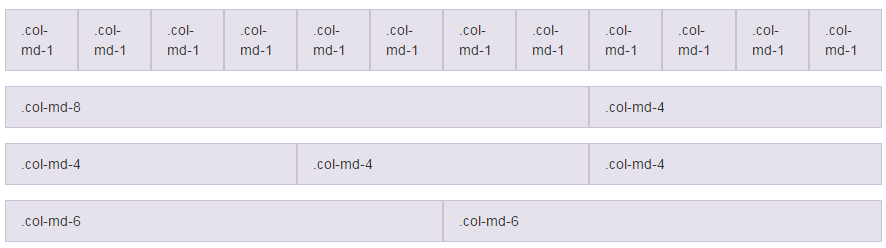
\includegraphics[width=\linewidth]{08/03_bootstrapGrid}
        \centering
        \caption{Exemble d'un contenidor bootstrap amb 4 files i diferent nombre de files}\label{img:gridSimple}
    \end{figure}

    La gràcia de dividir, cada fila en columnes és que en el moment que la grandària de la fila definida, superi la del dispositiu que les vol pintar, les columnes interiors de la fila s'apilen unes sobre les altres de forma automàtica, adaptant d'aquesta forma el contingut per un dispositiu mòbil sense necessitat de realitzar canvis en el codi o implementar un codi específic per aquests dispositius.

    La imatge\ref{img:gridAdapted} mostra com una configuració web per escriptori es reorganitzaria per un dispositiu mòbil.

    \begin{figure}[h]
        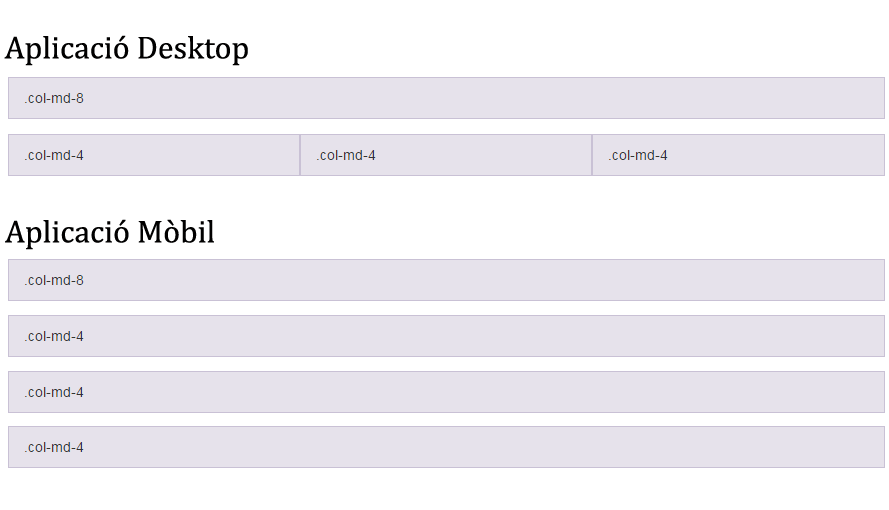
\includegraphics[width=\linewidth]{08/04_gridDesktopMobile}
        \centering
        \caption{Exemple del mateix grid en pantelles Escriptori i Mòbil}\label{img:gridAdapted}
    \end{figure}

    A part del grid, que representa la característica principal per la qual es va decidir utilitzar Bootstrap, aquesta entorn de treball també ofereix estils, o classes CSS, per taules, botons, formularis, imatges, tipografies, icones, barres de navegació, alertes, barres de progrés, contingut expansible i més funcionalitats.

    A pesar que la majoria de classes oferides per Bootstrap, han de ser retocades mitjançant CSS propi per tal d'encaixar i adaptar els diferents elements a la nostra aplicació web, representen un molt bon punt de partida, que estalvia temps als desenvolupadors i a la vegada, n'assegura la correcta visualització a través dels diferents dispositius.

    Resumint, el marc de treball Bootstrap proporciona principalment fitxers de codi CSS i Javascript que serveixen per complementar els nostres propis fitxers de codi. De la mateixa forma que les tecnologies CSS i Javascript, anteriorment descrites, aquest entorn de treball actua tant en el front-end del nostre sistema, com en el `back-end del front-end’. Per tant, exerceix a la vegada, un efecte a les capes Vista i Controlador de la nostra aplicació web.
